\subsection{Home Assistant}

Bei Home Assistant handelt es sich um Open Source Software im Bereich Smart Home. Es zielt darauf
ab, die Privatsphäre der Nutzenden zu erhöhen, indem so weit wie möglich auf externe Server
verzichtet wird. Typischerweise wird Home Assistant auf einem Raspberry Pi betrieben, der sich in
der gleichen Wohneinheit \todo{Haus / Wohnung?} mit den zu kontrollierenden Geräten befindet.
\parencite{homeassistantHomeAssistant}

Im Folgenden werden die wichtigsten Konzepte für das Verständnis von Home Assistant vorgestellt.
\textbf{Integrationen} stellen Software dar, welche mit anderen Plattformen kommuniziert, und es
somit ermöglicht, Geräte von verschiedenen Herstellern einzubinden. Daraufhin sind diese als
\textbf{Geräte} in Home Assistant vertreten und stellen sogenannte \textbf{Entitäten} bereit, welche
den Zustand des Geräts beschreiben und kontrollieren. Auf Basis von Sensoren und Kontroll-Entitäten
können nun \textbf{Automatisierungen} erstellt werden. Diese bestehen aus \textbf{Auslösern}, welche
die Automatisierung starten und etwas beschreiben, was im Haus\todo{?} passiert (Beispiel: "Person
betritt Wohnzimmer."). Des Weiteren können \textbf{Bedingungen} angegeben werden, die zusätzliche
Tests darstellen, welche die Ausführung der Automatisierung verhindern können (Beispiel:
"Umgebungslicht ist unter 20 Lux."). Sobald die Automatisierung ausgelöst wurde und die Bedingungen
übereinstimmen, werden \textbf{Aktionen} ausgeführt. Diese steuern Geräte oder Entitäten und werden
standardmäßig als Liste ausgeführt (Beispiel: "Leselampe anschalten, Musik abspielen.").
\textbf{Skripte} sind Sammlungen von Aktionen, welche als eine Aktion wiederverwendet werden können.
\parencite{homeassistantConceptsTerminology} Sowohl Automatisierungen als auch Skripte werden als
\acs{yaml}-Dateien\footnote{\acs{yaml}: \acl{yaml}} gespeichert und können über einen visuellen
Editor bearbeitet werden. Dieser wird im Folgenden betrachtet.

\subsubsection{Editor zum Erstellen von Automatisierungen}
\begin{figure}[!htb]
  \minipage{.49\textwidth}
  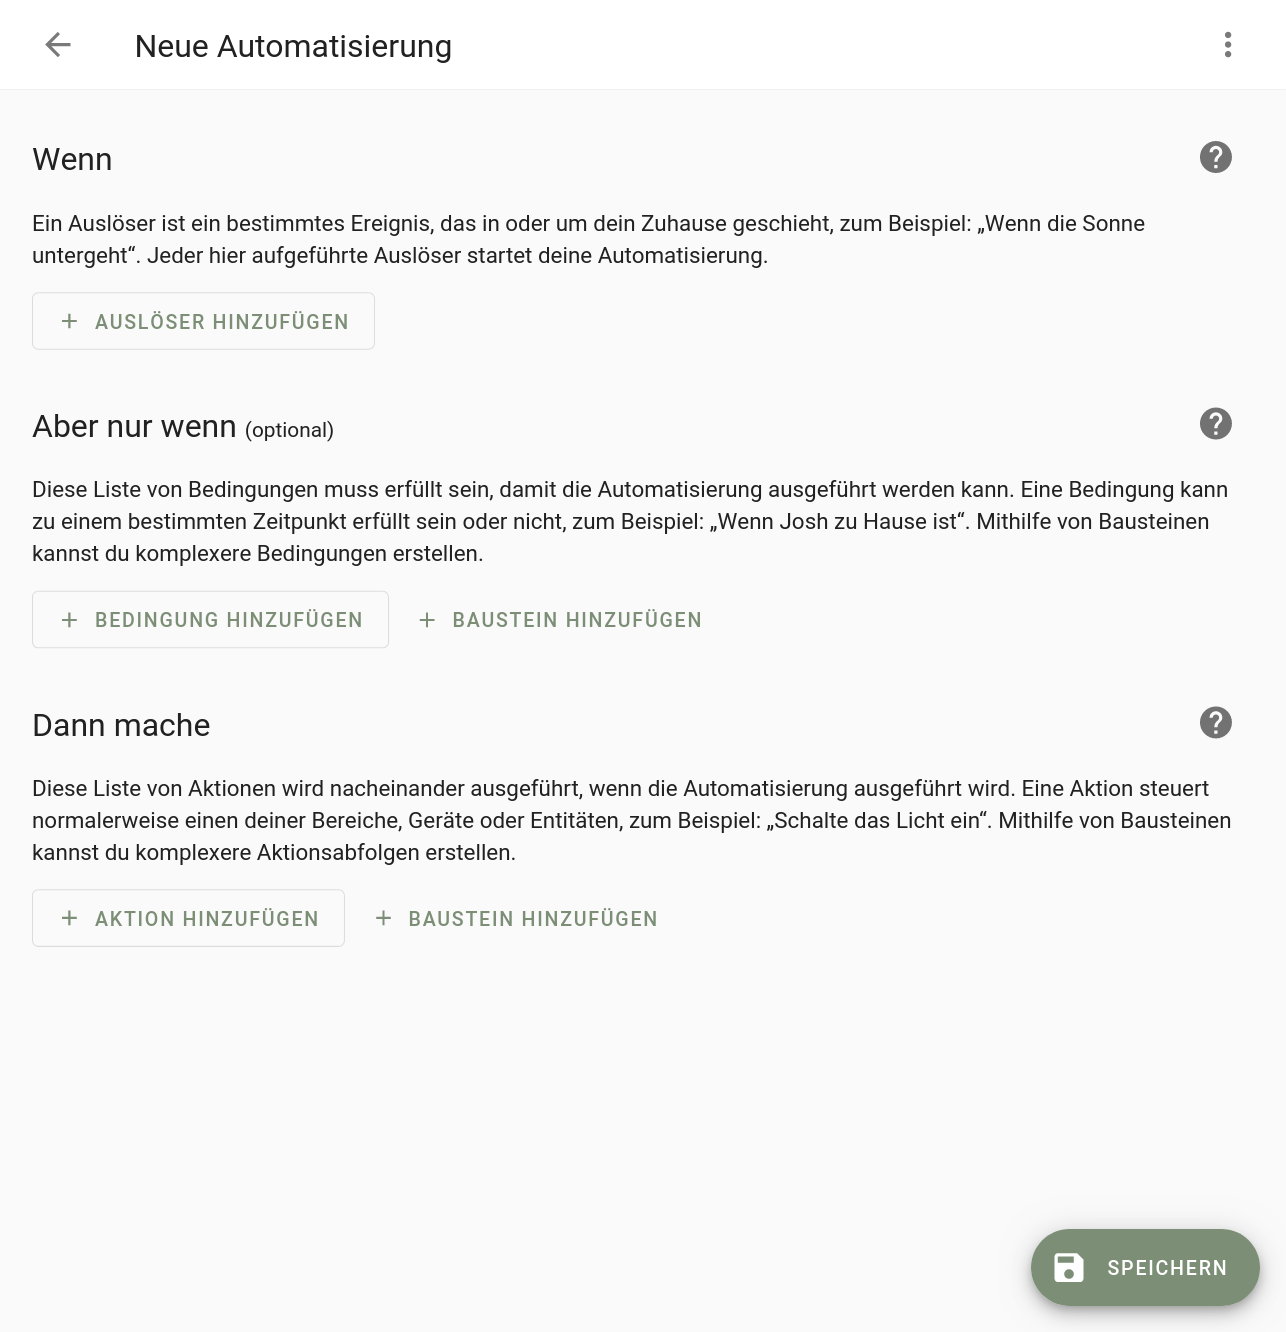
\includegraphics[width=\linewidth]{assets/hassio-automation-empty.png}
  \caption[]{Startpunkt der Erstellung einer Automatisierung in Home Assistant}
  \endminipage
  \hfill
  \minipage{.49\textwidth}
  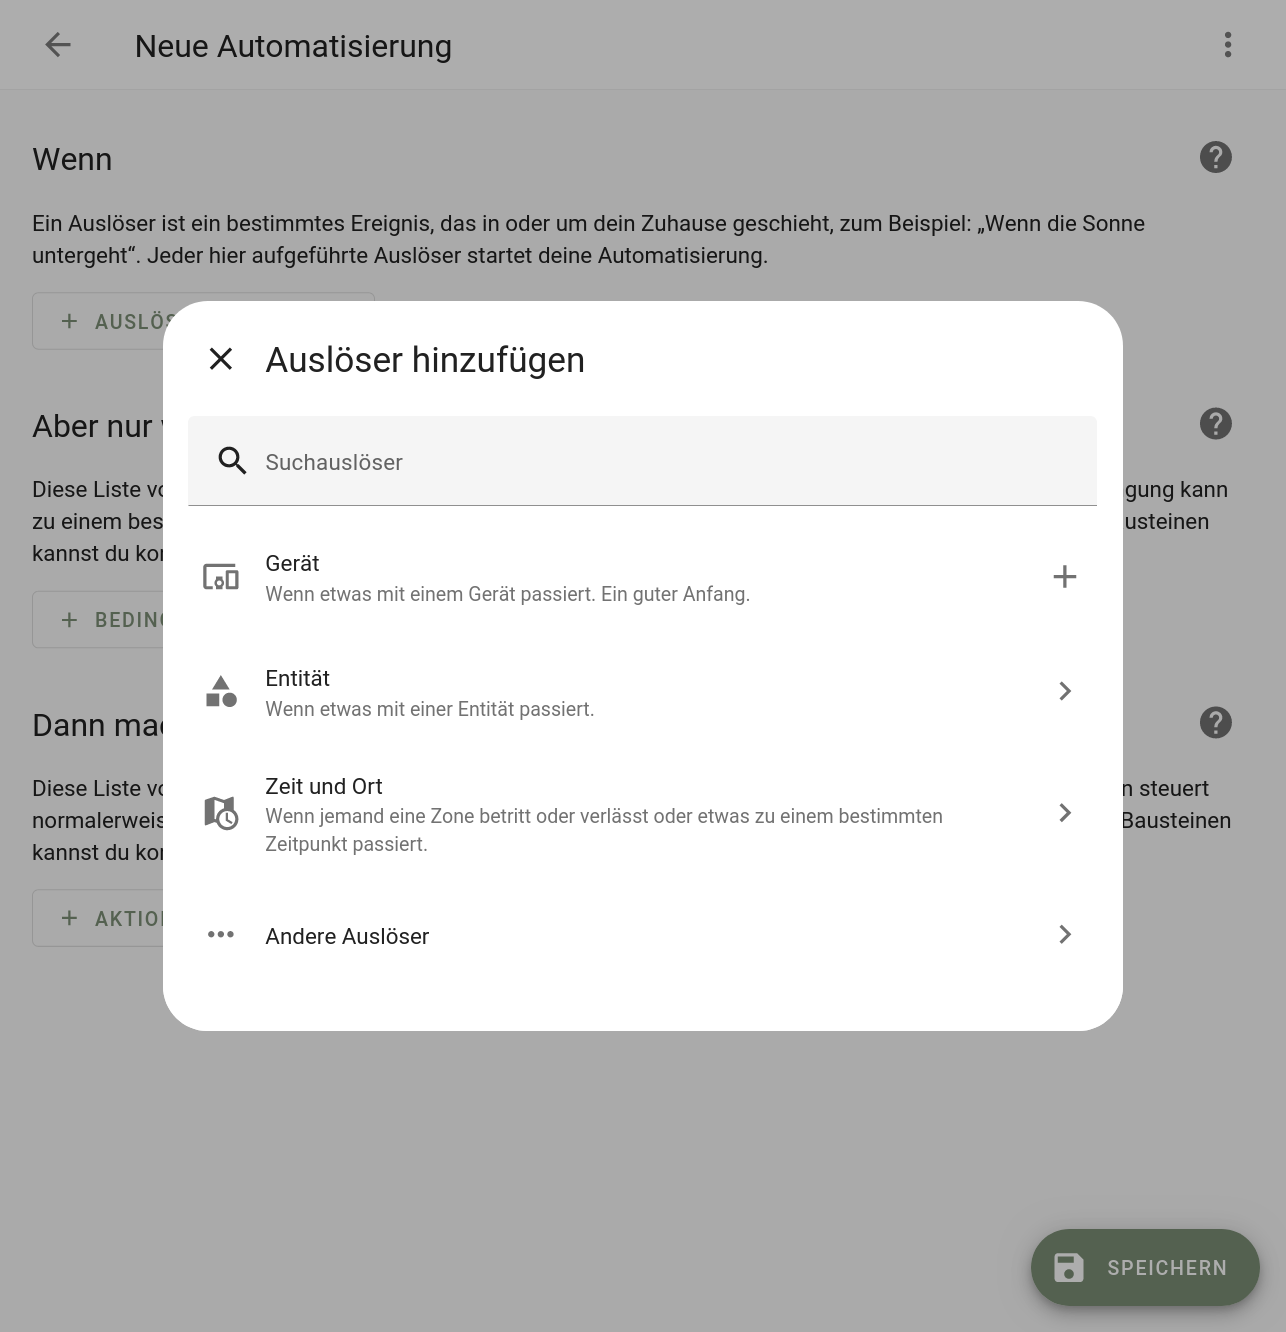
\includegraphics[width=\linewidth]{assets/hassio-automation-trigger-select-1.png}
  \caption{Auswahl eines Auslösers (1)}
  \endminipage
\end{figure}

\blindtext

\begin{figure}[!htb]
  \minipage{.49\textwidth}
  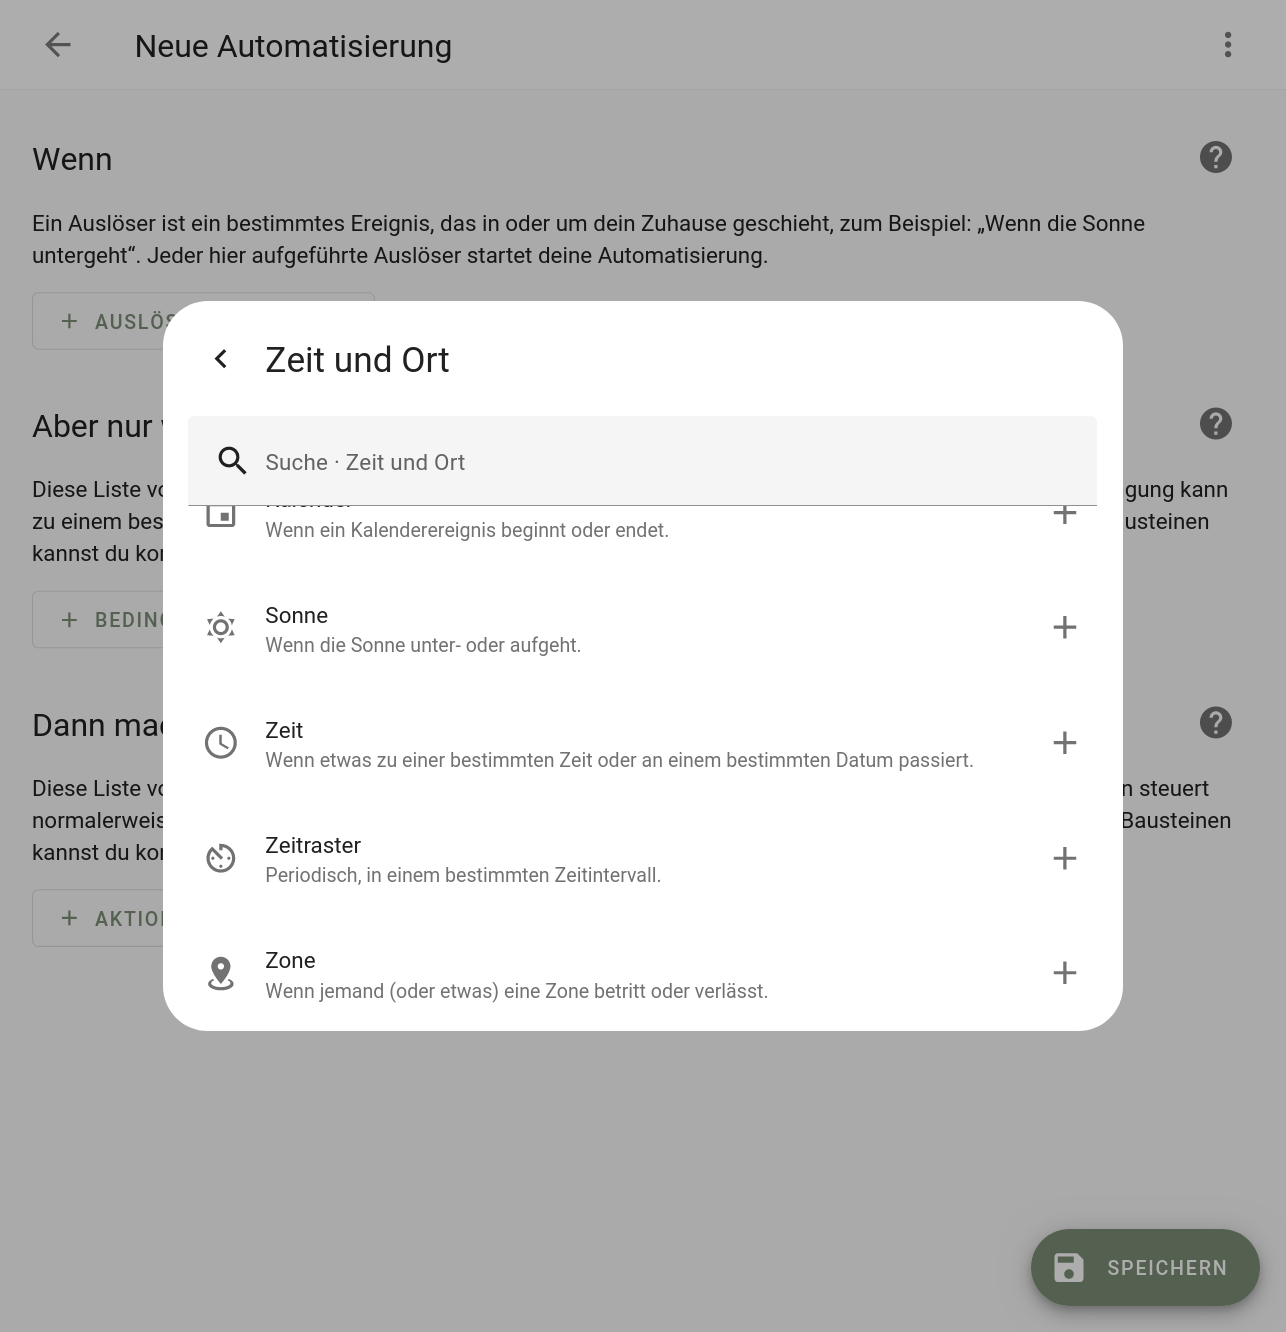
\includegraphics[width=\linewidth]{assets/hassio-automation-trigger-select-2.png}
  \caption{Auswahl eines Auslösers (2)}
  \endminipage
  \hfill
  \minipage{.49\textwidth}
  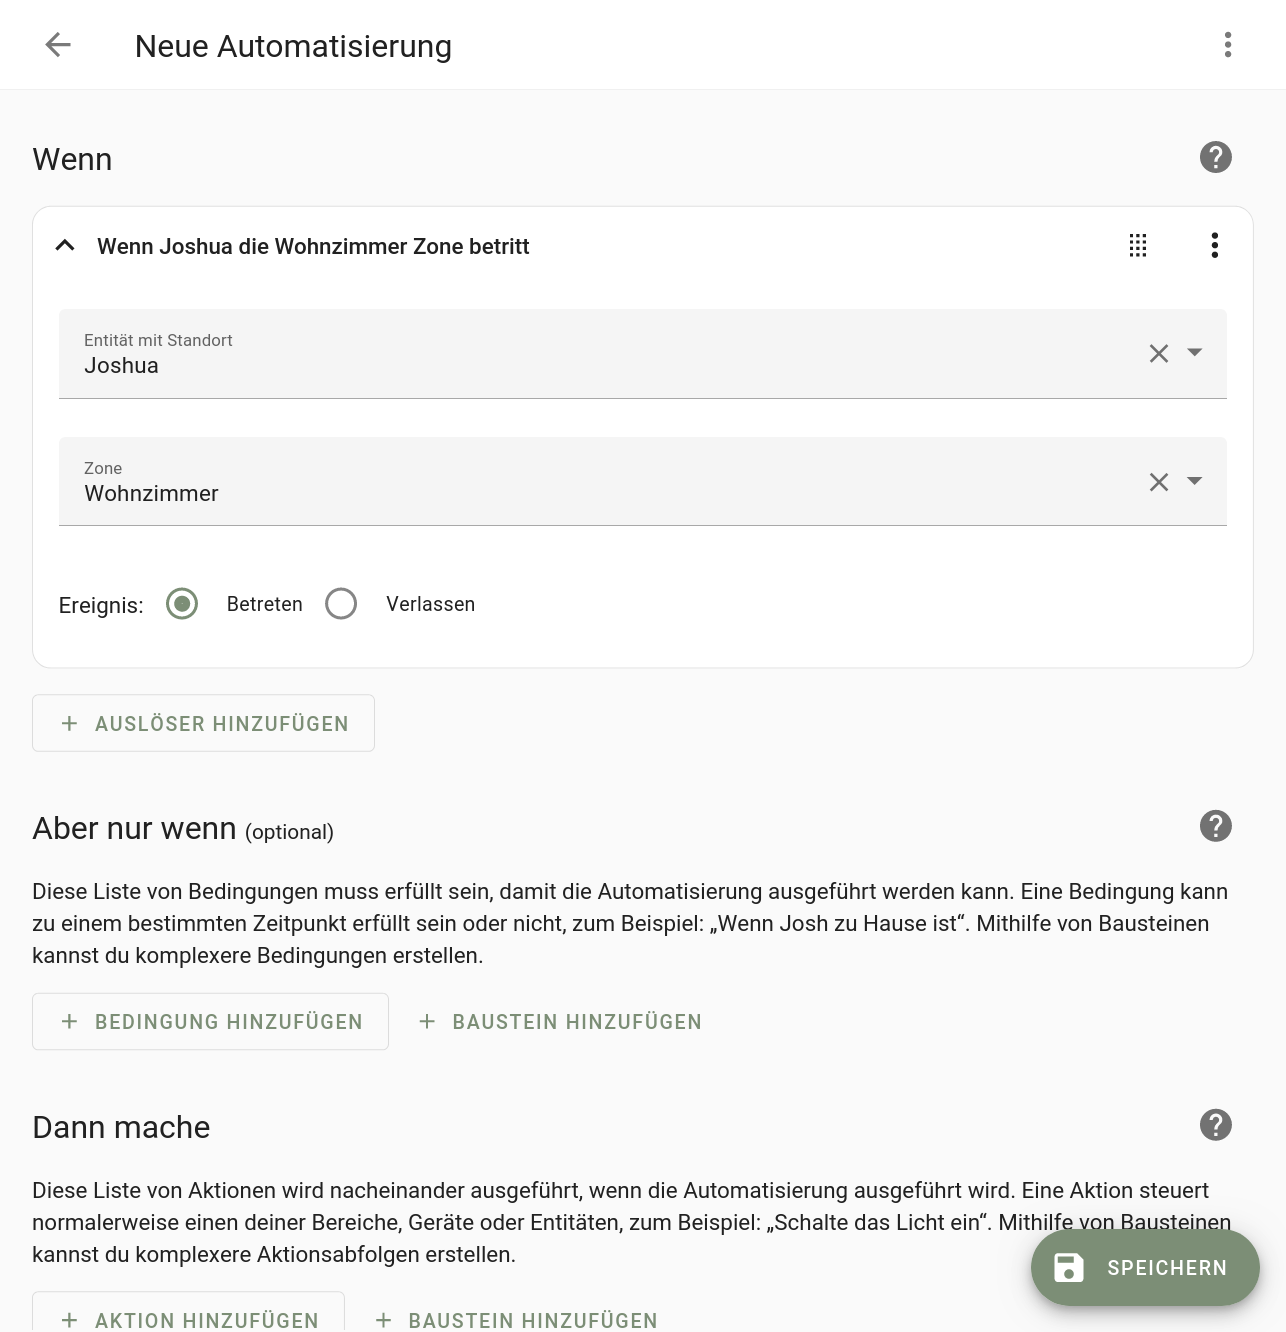
\includegraphics[width=\linewidth]{assets/hassio-automation-trigger.png}
  \caption{Angabe eines Auslösers in Home Assistant}
  \endminipage
\end{figure}

\blindtext

\begin{figure}[!htb]
  \minipage{.49\textwidth}
  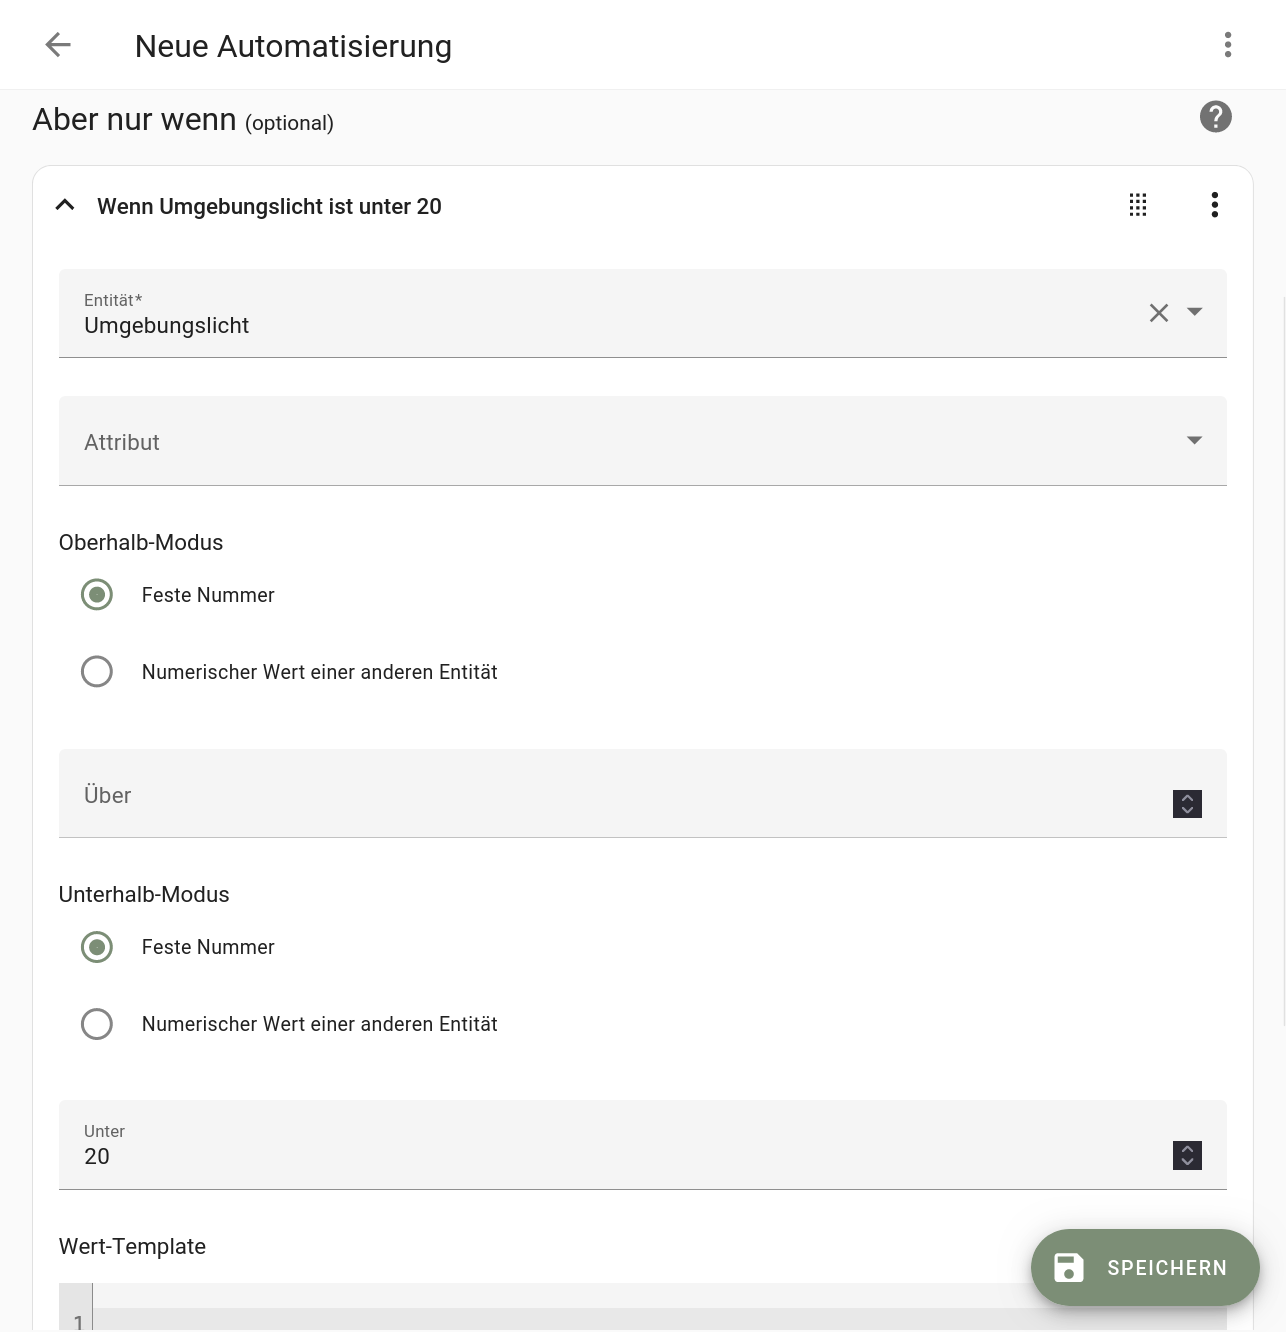
\includegraphics[width=\linewidth]{assets/hassio-automation-condition.png}
  \caption{Angabe einer Bedingung in Home Assistant}
  \endminipage
  \hfill
  \minipage{.49\textwidth}
  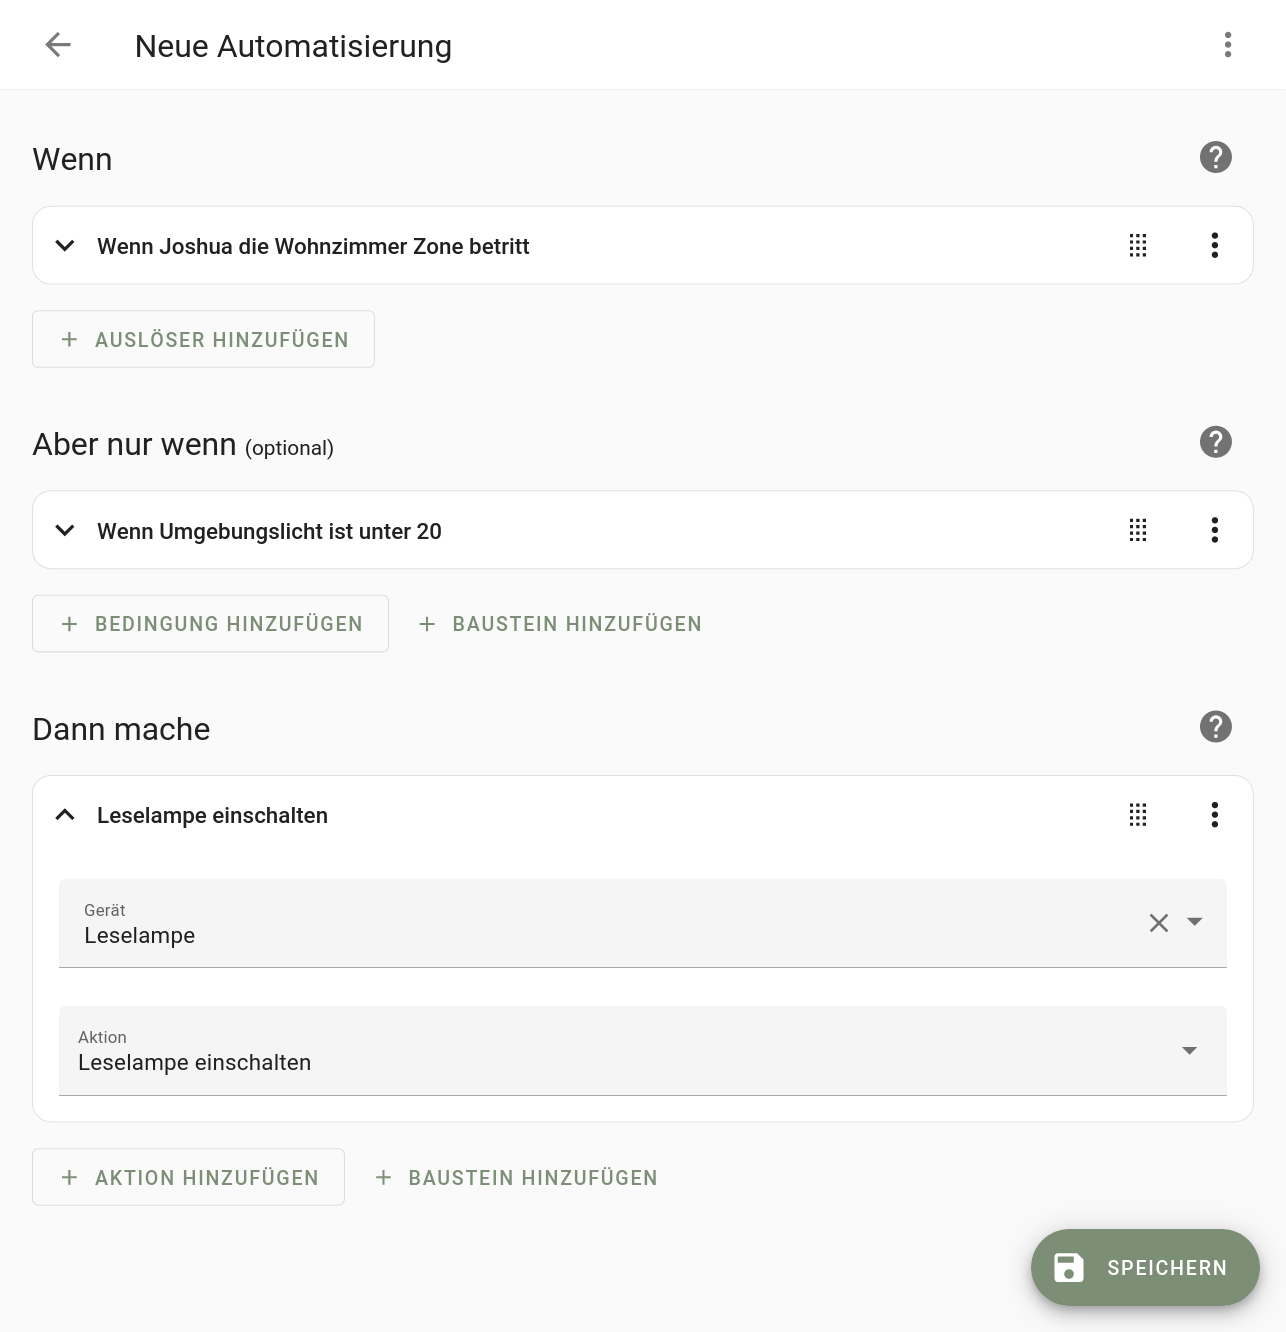
\includegraphics[width=\linewidth]{assets/hassio-automation-action.png}
  \caption{Angabe einer Aktion in Home Assistant}
  \endminipage
\end{figure}

\blindtext

\lstinputlisting[
  label=lst:automation,
  caption={\ac{yaml}-Definition einer Automatisierung in Home Assistant},
  language=yaml
]{assets/hassio-automation.yaml}
